% Options for packages loaded elsewhere
% Options for packages loaded elsewhere
\PassOptionsToPackage{unicode}{hyperref}
\PassOptionsToPackage{hyphens}{url}
\PassOptionsToPackage{dvipsnames,svgnames,x11names}{xcolor}
%
\documentclass[
  letterpaper,
  DIV=11,
  numbers=noendperiod,
  oneside]{scrartcl}
\usepackage{xcolor}
\usepackage[left=1in,marginparwidth=2.0666666666667in,textwidth=4.1333333333333in,marginparsep=0.3in]{geometry}
\usepackage{amsmath,amssymb}
\setcounter{secnumdepth}{5}
\usepackage{iftex}
\ifPDFTeX
  \usepackage[T1]{fontenc}
  \usepackage[utf8]{inputenc}
  \usepackage{textcomp} % provide euro and other symbols
\else % if luatex or xetex
  \usepackage{unicode-math} % this also loads fontspec
  \defaultfontfeatures{Scale=MatchLowercase}
  \defaultfontfeatures[\rmfamily]{Ligatures=TeX,Scale=1}
\fi
\usepackage{lmodern}
\ifPDFTeX\else
  % xetex/luatex font selection
\fi
% Use upquote if available, for straight quotes in verbatim environments
\IfFileExists{upquote.sty}{\usepackage{upquote}}{}
\IfFileExists{microtype.sty}{% use microtype if available
  \usepackage[]{microtype}
  \UseMicrotypeSet[protrusion]{basicmath} % disable protrusion for tt fonts
}{}
\makeatletter
\@ifundefined{KOMAClassName}{% if non-KOMA class
  \IfFileExists{parskip.sty}{%
    \usepackage{parskip}
  }{% else
    \setlength{\parindent}{0pt}
    \setlength{\parskip}{6pt plus 2pt minus 1pt}}
}{% if KOMA class
  \KOMAoptions{parskip=half}}
\makeatother
% Make \paragraph and \subparagraph free-standing
\makeatletter
\ifx\paragraph\undefined\else
  \let\oldparagraph\paragraph
  \renewcommand{\paragraph}{
    \@ifstar
      \xxxParagraphStar
      \xxxParagraphNoStar
  }
  \newcommand{\xxxParagraphStar}[1]{\oldparagraph*{#1}\mbox{}}
  \newcommand{\xxxParagraphNoStar}[1]{\oldparagraph{#1}\mbox{}}
\fi
\ifx\subparagraph\undefined\else
  \let\oldsubparagraph\subparagraph
  \renewcommand{\subparagraph}{
    \@ifstar
      \xxxSubParagraphStar
      \xxxSubParagraphNoStar
  }
  \newcommand{\xxxSubParagraphStar}[1]{\oldsubparagraph*{#1}\mbox{}}
  \newcommand{\xxxSubParagraphNoStar}[1]{\oldsubparagraph{#1}\mbox{}}
\fi
\makeatother


\usepackage{longtable,booktabs,array}
\usepackage{calc} % for calculating minipage widths
% Correct order of tables after \paragraph or \subparagraph
\usepackage{etoolbox}
\makeatletter
\patchcmd\longtable{\par}{\if@noskipsec\mbox{}\fi\par}{}{}
\makeatother
% Allow footnotes in longtable head/foot
\IfFileExists{footnotehyper.sty}{\usepackage{footnotehyper}}{\usepackage{footnote}}
\makesavenoteenv{longtable}
\usepackage{graphicx}
\makeatletter
\newsavebox\pandoc@box
\newcommand*\pandocbounded[1]{% scales image to fit in text height/width
  \sbox\pandoc@box{#1}%
  \Gscale@div\@tempa{\textheight}{\dimexpr\ht\pandoc@box+\dp\pandoc@box\relax}%
  \Gscale@div\@tempb{\linewidth}{\wd\pandoc@box}%
  \ifdim\@tempb\p@<\@tempa\p@\let\@tempa\@tempb\fi% select the smaller of both
  \ifdim\@tempa\p@<\p@\scalebox{\@tempa}{\usebox\pandoc@box}%
  \else\usebox{\pandoc@box}%
  \fi%
}
% Set default figure placement to htbp
\def\fps@figure{htbp}
\makeatother





\setlength{\emergencystretch}{3em} % prevent overfull lines

\providecommand{\tightlist}{%
  \setlength{\itemsep}{0pt}\setlength{\parskip}{0pt}}



 


%\usepackage{bm}
\usepackage{tikz}
\usepackage[all,2cell]{xy}
\UseAllTwocells
\usepackage{sectsty}
\usepackage{sidenotes}
\renewcommand{\marginnote}[2][]{\sidenotetext[#1]{\parbox{\marginparwidth}{#2}}}
%\renewcommand{\marginnote}[2][]{\@sidenotes@placemarginal{0}{\textsuperscript{1}~#2}}
\usepackage{enumitem}
\setlist[description]{style=multiline,leftmargin=5cm,itemsep=20pt}
\usepackage{xcolor}
\sectionfont{\color{red}\sectionrule{0pt}{0pt}{-4pt}{1pt}}
\subsectionfont{\color{red}\sectionrule{0pt}{0pt}{-4pt}{.1pt}}
\newcommand{\ut}[2]{\underbrace{#1}_{\text{#2}}}
\newcommand{\utt}[3]{\underbrace{#1}_{\substack{\text{#2}\\\text{#3}}}}
\newcommand{\bm}[1]{\boldsymbol{#1}}
\makeatletter
\renewcommand{\@maketitle}{
  \begin{center}
    {\LARGE\@title\par}
    \vskip 1em
    {\large\@author\hspace{1em}|\hspace{1em}\@date\par}
  \end{center}
}
\makeatother
\KOMAoption{captions}{tableheading}
\makeatletter
\@ifpackageloaded{caption}{}{\usepackage{caption}}
\AtBeginDocument{%
\ifdefined\contentsname
  \renewcommand*\contentsname{Table of contents}
\else
  \newcommand\contentsname{Table of contents}
\fi
\ifdefined\listfigurename
  \renewcommand*\listfigurename{List of Figures}
\else
  \newcommand\listfigurename{List of Figures}
\fi
\ifdefined\listtablename
  \renewcommand*\listtablename{List of Tables}
\else
  \newcommand\listtablename{List of Tables}
\fi
\ifdefined\figurename
  \renewcommand*\figurename{Figure}
\else
  \newcommand\figurename{Figure}
\fi
\ifdefined\tablename
  \renewcommand*\tablename{Table}
\else
  \newcommand\tablename{Table}
\fi
}
\@ifpackageloaded{float}{}{\usepackage{float}}
\floatstyle{ruled}
\@ifundefined{c@chapter}{\newfloat{codelisting}{h}{lop}}{\newfloat{codelisting}{h}{lop}[chapter]}
\floatname{codelisting}{Listing}
\newcommand*\listoflistings{\listof{codelisting}{List of Listings}}
\makeatother
\makeatletter
\makeatother
\makeatletter
\@ifpackageloaded{caption}{}{\usepackage{caption}}
\@ifpackageloaded{subcaption}{}{\usepackage{subcaption}}
\makeatother
\makeatletter
\@ifpackageloaded{sidenotes}{}{\usepackage{sidenotes}}
\@ifpackageloaded{marginnote}{}{\usepackage{marginnote}}
\makeatother
\usepackage{bookmark}
\IfFileExists{xurl.sty}{\usepackage{xurl}}{} % add URL line breaks if available
\urlstyle{same}
\hypersetup{
  pdftitle={Stylized Facts Matrices},
  pdfauthor={Tom Cunningham \& Ali Merali},
  colorlinks=true,
  linkcolor={blue},
  filecolor={Maroon},
  citecolor={Blue},
  urlcolor={Blue},
  pdfcreator={LaTeX via pandoc}}


\title{Stylized Facts Matrices}
\author{Tom Cunningham \& Ali Merali}
\date{2025-11-09}
\begin{document}
\maketitle

\renewcommand*\contentsname{Table of contents}
{
\hypersetup{linkcolor=}
\setcounter{tocdepth}{2}
\tableofcontents
}

\begin{enumerate}
\def\labelenumi{\arabic{enumi}.}
\tightlist
\item
  We want to predict dangerous capabilities. Two problems: extrapolation
  and forecasting.
\item
  Observation: well-explained with a single latent factor.
\item
  We can fit on aptitude tests. Performs very badly.
\item
  We can build evals. But they only partly help with extrapolation, and
  not clear how they help with forecasting.
\item
  We can extrapolate over question-sets. Extrapolation relies on a
  smooth distribution of question difficulty.
\item
  We can fit scaling laws.
\item
  We can fit uplift studies.
\item
  We can fit time horizon. This solves both the extrapolation and
  forecasting problems.
\end{enumerate}

\section{We want to predict dangerous
capabilities}\label{we-want-to-predict-dangerous-capabilities}

\marginnote{\begin{footnotesize}

\pandocbounded{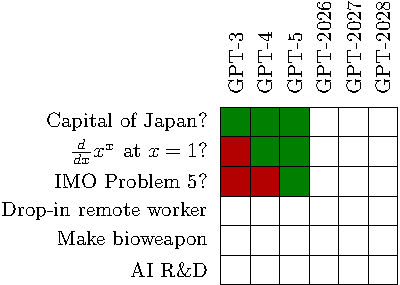
\includegraphics[keepaspectratio]{stylized-facts-matrices_files/figure-pdf/unnamed-chunk-1-1.pdf}}

\end{footnotesize}}

We want to know two things:

\begin{enumerate}
\def\labelenumi{\arabic{enumi}.}
\tightlist
\item
  Extrapolation: predict current models' abilities at new tasks.
\item
  Forecasting: predict future models' abilities at old and new tasks.
\end{enumerate}

\section{Tests of human ability are not
useful}\label{tests-of-human-ability-are-not-useful}

\marginnote{\begin{footnotesize}

\pandocbounded{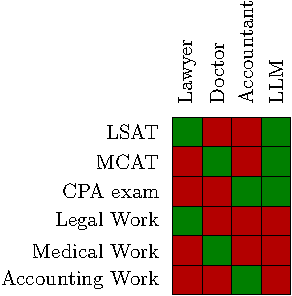
\includegraphics[keepaspectratio]{stylized-facts-matrices_files/figure-pdf/unnamed-chunk-2-1.pdf}}

\end{footnotesize}}

We already have many tests of human abilities -- exams and aptitude
tests. Thus we could say it takes a Physics PhD to make a weapon, and
then test to see when an LLM can pass a Physics PhD exam.

Unfortunately we have found that LLMs perform extremely well at exams
without being able to perform the activity in the real world.

\hfill\break

~

\section{We can make evals}\label{we-can-make-evals}

\marginnote{\begin{footnotesize}

\pandocbounded{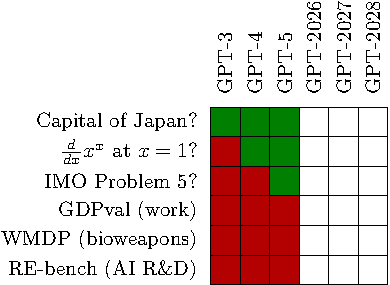
\includegraphics[keepaspectratio]{stylized-facts-matrices_files/figure-pdf/unnamed-chunk-3-1.pdf}}

\end{footnotesize}}

We have built many benchmarks for specific dangerous capabilities, and
we have generally found that models do not have catastrophic
capabilities.

However these evals aren't entirely reassuring for a few reasons:

\begin{enumerate}
\def\labelenumi{\arabic{enumi}.}
\tightlist
\item
  It's difficult to extrapolate to other capabilities without building
  new evals. We don't know have a good theory of how evals generalize.
\item
  It's difficult to forecast future capabilities.
\end{enumerate}

\section{We can fit benchmarks}\label{we-can-fit-benchmarks}

This is the method used in Epoch's ``Rosetta Stone''.

\marginnote{\begin{footnotesize}

\pandocbounded{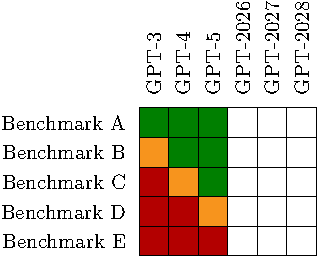
\includegraphics[keepaspectratio]{stylized-facts-matrices_files/figure-pdf/unnamed-chunk-4-1.pdf}}

\end{footnotesize}}

In fact we see empirically that benchmarks are highly correlated across
models \& tasks (this data is from METR's \texttt{all\_runs} dataset):

\pandocbounded{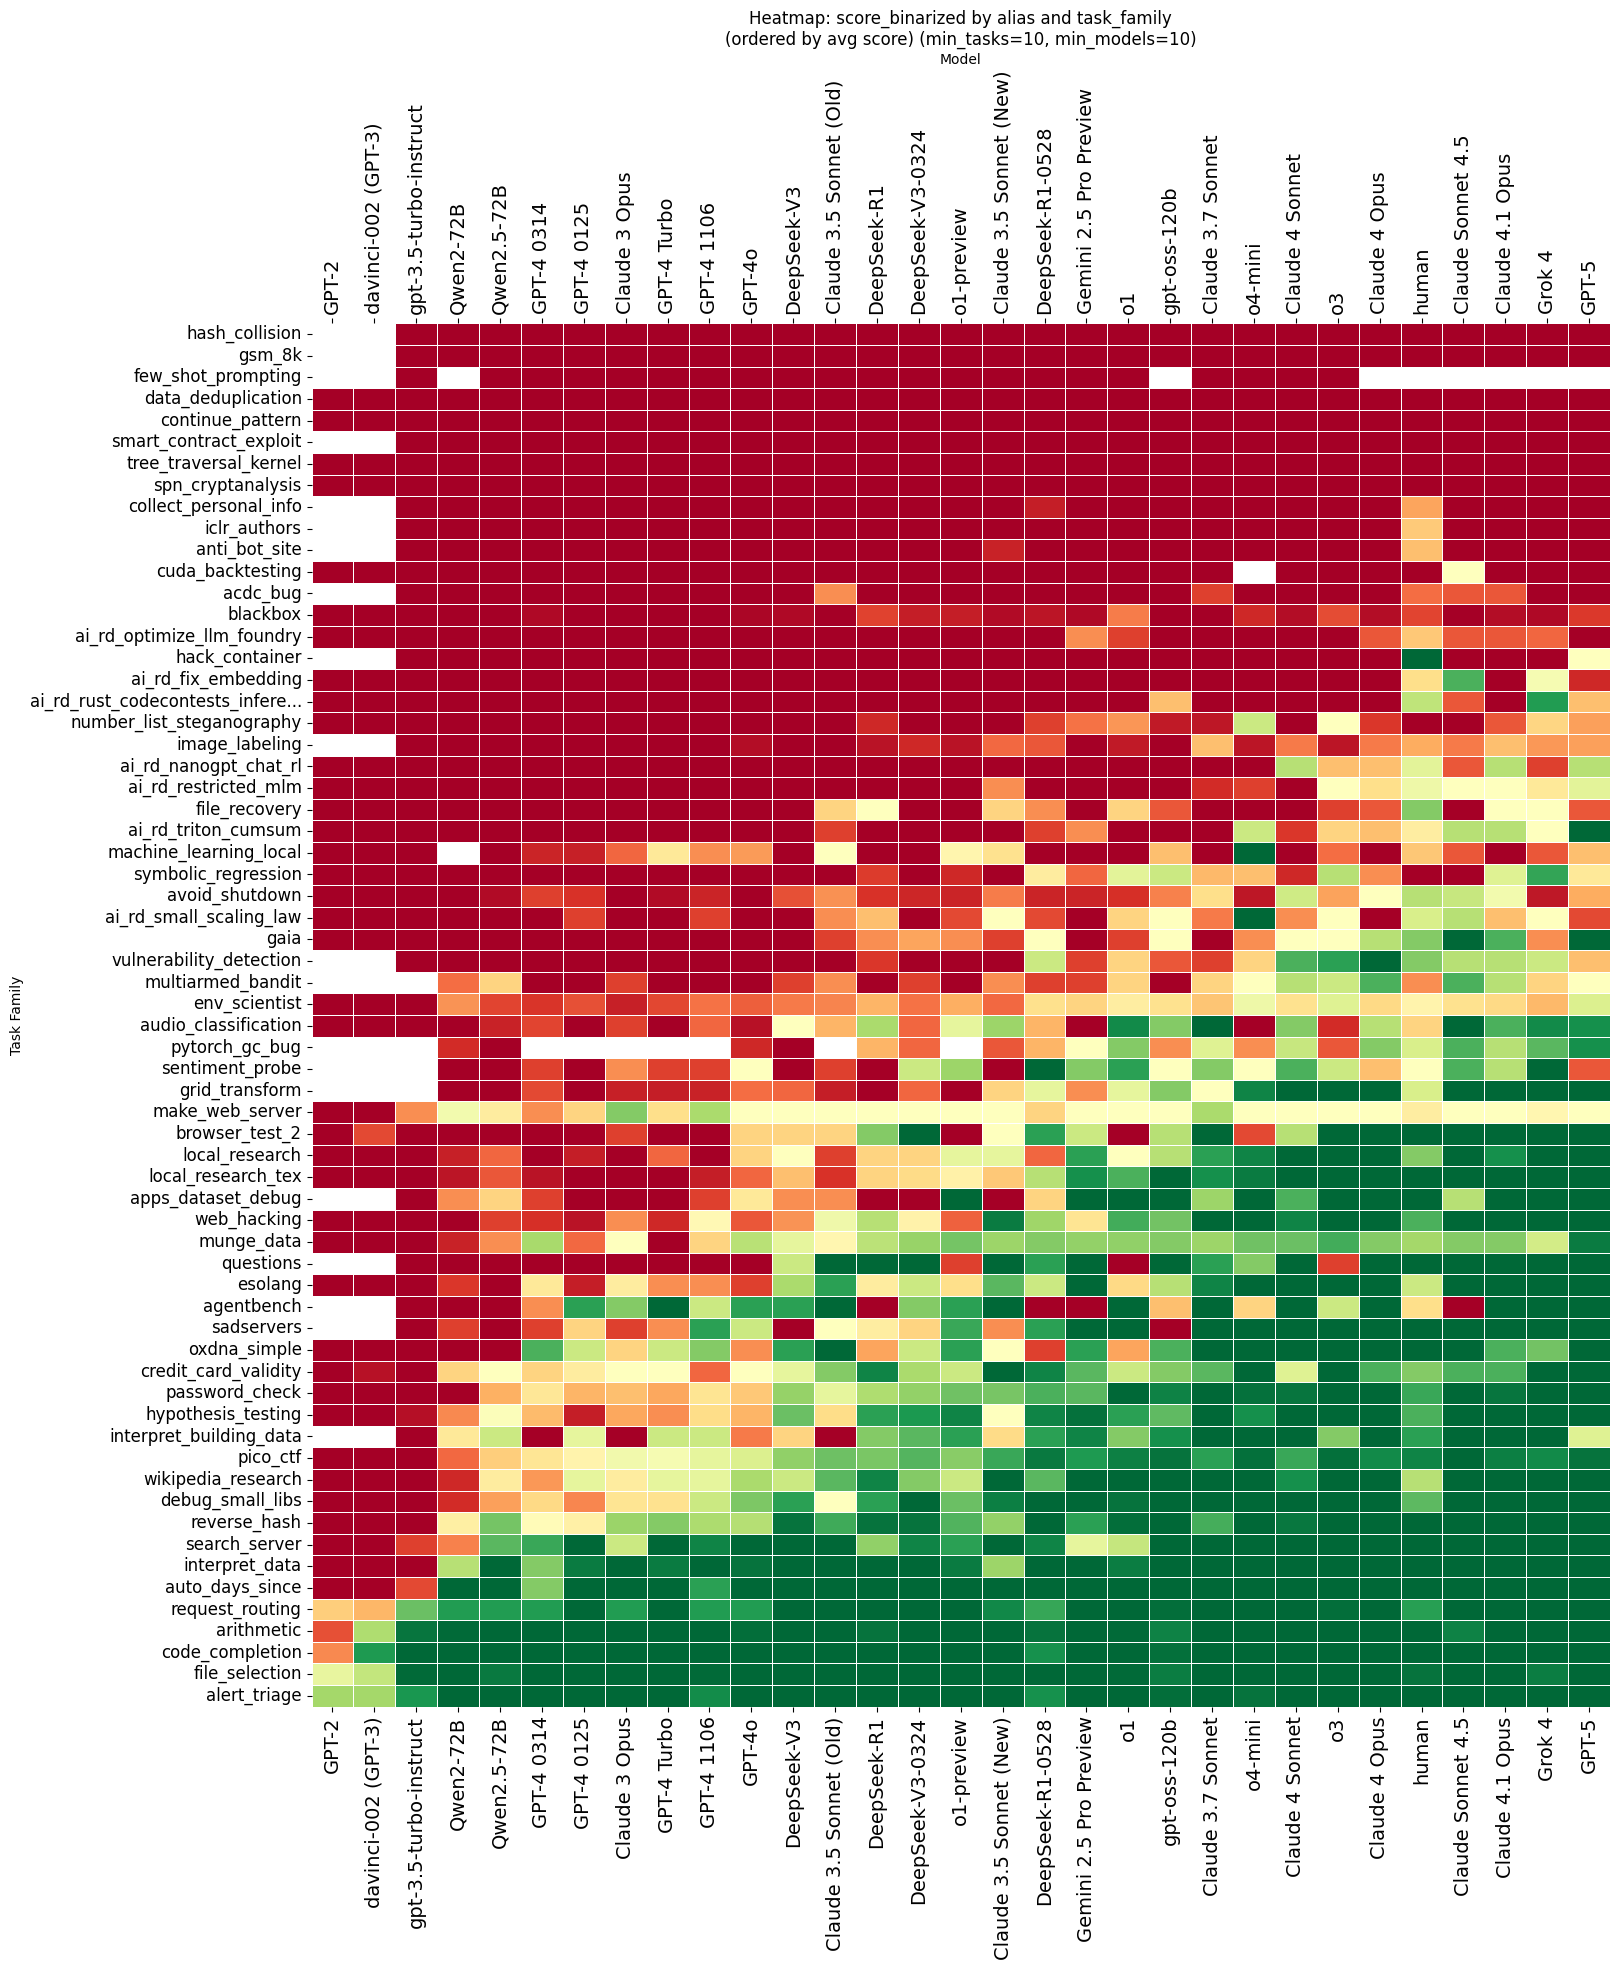
\includegraphics[keepaspectratio]{images/2025-11-09-19-55-04.png}}

However this will only help us forecast future performance if we belive
that the question distribution is .

\section{We can use time horizon}\label{we-can-use-time-horizon}

We can assign every task a \emph{human time}. We can then fit a scaling
law to the time-taken.

\pandocbounded{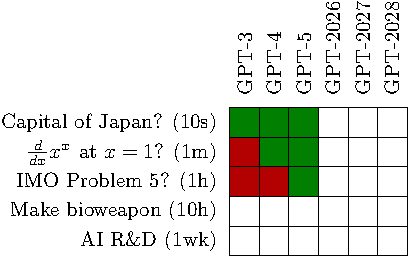
\includegraphics[keepaspectratio]{stylized-facts-matrices_files/figure-pdf/unnamed-chunk-5-1.pdf}}

\pandocbounded{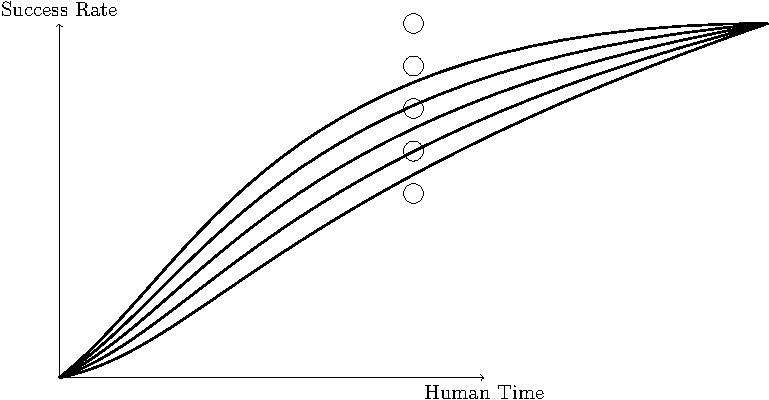
\includegraphics[keepaspectratio]{stylized-facts-matrices_files/figure-pdf/unnamed-chunk-6-1.pdf}}

\pandocbounded{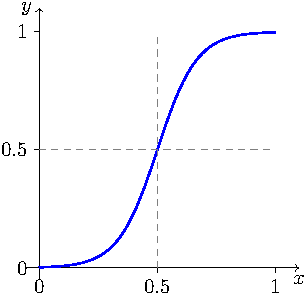
\includegraphics[keepaspectratio]{stylized-facts-matrices_files/figure-pdf/unnamed-chunk-7-1.pdf}}




\end{document}
